\chapter{Using LaTeX to make documents that meet NREL's requirements}
A series of LaTeX class files called \emph{NREL...cls} have been written to implement NREL's formatting requirements in LaTeX. Authors are required to use these class files to create NREL documents.

\section{NREL's LaTeX Environment}
\subsection{Web Interface}
NREL authors are strongly encouraged to use the NREL-hosted web-based latex environment to produce documents from LaTeX. This can be found at \href{latex.nrel.gov}{latex.nrel.gov}. More information can be found at \href{latex.nrel.gov}{latex.nrel.gov}.

Advantages of \href{latex.nrel.gov}{latex.nrel.gov} include:
\begin{enumerate}
\item No need to maintain a local version of LaTeX
\item Everyone uses the same version of LaTeX
\item Editors and reviewers can work in a user-friendly environment
\item There is an always-on ``track changes'' feature
\item Secure hosting of documents within the NREL domain
\item Ability to download source documents for archiving
\end{enumerate}

\subsection{Starting new documents}
\begin{enumerate}
\item Go to \href{https://github.com/NREL/latex_editing}{https://github.com/NREL/latex\_editing} and download the repository as a .zip file from the icon on the lower right hand side of the page.
\item Got to \href{latex.nrel.gov}{latex.nrel.gov} and start a new project by uploading the zip file. Modify the project properties (name, collaborators, etc) as required.
\item Modify \emph{main.tex} as required.
\end{enumerate}

Authors are welcome to use their own installation of LaTeX to prepare a document using the \emph{nrel.cls} file, but should note that they will need to transfer the document to \href{latex.nrel.gov}{latex.nrel.gov} at some point.

\subsection{Working with pubhub}
NREL uses a web-based publications management system that can be found at \href{pubhub.nrel.gov}{pubhub.nrel.gov}. This system should be used in different ways, depending on the stage that the document is at.
\begin{itemize}
\item Editing documents: 
\begin{itemize} 
\item Authors check in the PDF and provide a link to the \href{latex.nrel.gov}{latex.nrel.gov} document.
\item Authors add the latex.editor@nrel.gov user to their document
\item The editor logs in to the latex.editor@nrel.gov account on \href{latex.nrel.gov}{latex.nrel.gov} to make edits. The author may need to support some modifications. Comments should be added on a new line after the \% symbol, and will be found by the ``track changes'' feature.
\end{itemize}
\item Reviewing documents:
\begin{itemize} 
\item Approvers can work on either the PDF or the LaTeX document, noting that working on the \href{latex.nrel.gov}{latex.nrel.gov} document requires an internet connection.
\end{itemize}
\item Final documents: 
\begin{itemize} 
\item All files used to prepare the latex document should be downloaded from \href{latex.nrel.gov}{latex.nrel.gov} and stored in pubhub once the final document has been published.
\end{itemize}
\end{itemize}

\subsection{FAQs for working with latex.nrel.gov}
A separate FAQ that is updated regularly is available to NREL users at \href{latex.nrel.gov}{latex.nrel.gov}.

\section{NREL class files}\label{sec:nrelcls}
Class files control the formatting and presentation of documents. Several have been written that format documents so that they meet NREL's requirements. The class files currently available include:
\begin{description}
\item[NRELreport.cls]{compiles the document using the LaTeX \emph{report} class, with NREL formatting. This is intended for longer documents and allows the use of chapters.}
\item[NRELarticle.cls] compiles the document using the LaTeX \emph{article} class, with NREL formatting. This is intended for shorter documents such as journal articles. This class does not support the use of chapters.
\end{description}

As with normal classes, options are passed to the class in the \verb+\documentclass+ line:

\begin{lstlisting}
\documentclass[option1,...,optionn]{nrel}
\end{lstlisting}

NREL-specific options include:
\begin{description}
\item[draft]{add a `draft' watermark to all pages and colours all links in blue.}
\item[tagged]{create a tagged PDF}
\end{description}

The \emph{NREL....cls} files call a variety of other packages. Packages are codes that modify the appearance or behaviour of LaTeX to achieve something. Table \ref{Tab:Packages} lists the packages that are explicitly called by \emph{nrel.cls} in the order they are called in. These packages often call other packages, so this is not an exhaustive list.

\begin{table*}[!h]
\centering
\caption[Packages loaded by the NREL classes]{Packages loaded by the NREL classes.}
\label{Tab:Packages}
\begin{tabular*}{\textwidth}{llp{0.6\textwidth}}
\toprule
Package & Options & Functionality\\
\midrule
%accessibility & tagged & generates the document structure and tagging \\
amsfonts, amssymb & & supplies AMS fonts, which are useful for mathematics \\
babel & english & activates language-appropriate hyphenation rules\\
booktabs & & improves the formatting of tables \\
caption & & required to generate captions for floats\\
courier& & changes fonts \\
fontenc & T1 & enables direct typing of international characters \\
geometry & & sets page size and margins \\
graphicx & & graphics handling, including \emph{.eps} figures \\
helvet& scaled=0.83 & sets helvetica as the default sans-serif font, with correct scaling to match the serif font size\\
hyphenat & & improves spacing and breaking of hyphenated words \\
listings & & enables the inclusion of high-quality computer code listings\\
mathptmx& & changes fonts \\
nag & & checks that packages are up to date and looks for bad habits in LaTeX code. \\
parskip & & required for better spacing\\
pdfcomment & & required for tool-tips. Also calls the \texttt{hyperref} package  \\
setspace & & required for better spacing\\
subcaption & & provides the \texttt{subfigure} environment to produce sub figures \\
tocloft & & improved table of contents and list of figures/tables in memoir documents\\
tocbibind & nottoc, notlot, notlof & Add bibliography/index/contents to Table of Contents in memoir documents\\
todonotes & & inline and margin to-do notes \\
xcolor & & Driver-independent color extensions for LaTeX and pdfLaTeX\\
\bottomrule
\end{tabular*}
\end{table*}

It should be noted that the `english` option to Babel really means \emph{American} English.

\section{Creating Content}
\subsection{Front, main, and back matter}
NREL's convention is to have Roman numerals in the front matter, and then arabic numerals in the main matter of the document (after the tables of contents, figures and tables). Tables and figures in the front matter are also numbered differently (Table A, B, C, ...) than in the main matter (Table 1, 2, 3, ...).

This change in page and float numbering is implemented using the \verb+\frontmatter+, \verb+\mainmatter+, and \verb+\backmatter+ commands at the start of these sections of the document:

\begin{lstlisting}
\begin{document}

\maketitle
\frontmatter
...
\tableofcontents
\clearpage
\listoffigures
\listoftables
\mainmatter
...
\backmatter
\end{document}
\end{lstlisting}

Page numbering in the front matter (i.e. the Abstract, Summary, and Foreword chapters or sections) starts at page 3 to allow for NREL cover pages.

If you don't use the \verb+\frontmatter+ commands, you may need to increment the page counter manually. To increment the counter $n$ pages, use \verb+\setcounter{page}{n}+ after \verb+\begin{document}+.

\subsection{Cross references}
Use labels and references to refer back and forth to figures, equations, tables and sections. 

For example, an equation can be added using the following text:

\begin{lstlisting}
\begin{equation}
y = mx+c
\label{eqn:line}
\end{equation}
\end{lstlisting}

This gives the following:
\begin{equation}
y = mx+c
\label{eqn:line}
\end{equation}

And using the text \verb+Eqn. \ref{eqn:line}+ provides a cross reference to Eqn. \ref{eqn:line}.

\subsection{Floats}
Floats are images, tables or other pieces of the document that are free to move to the best place in the document for them. The two most common floats are the tabular environment (for tables) and the figure environment for figures.

\subsubsection{Tables}
Use the \texttt{tabular} environment to produce basic tables. Table~\ref{tab:widgets} is produced using this code: 

\begin{lstlisting}
\begin{table}[!h]
\centering
\caption{An example table.}\label{tab:widgets}
\begin{tabular}{lr}
Item & Quantity \\
\hline
Widgets & 42 \\
Gadgets & 13
\end{tabular}
\end{table}
\end{lstlisting}

\begin{table}[!h]
\centering
\caption{An example table.}\label{tab:widgets}
\begin{tabular}{lr}
Item & Quantity \\
\hline
Widgets & 42 \\
Gadgets & 13
\end{tabular}
\end{table}

If all of the delimiters (\&) are included in each row, the table will be complete and will produce a better PDF.

Note that tables produced using the \texttt{tabular} and \texttt{tabular*} environments are automatically typeset in a sans-serif font which is similar to Arial. This is required by the NREL style guide.

\subsubsection{Figures}
To include a figure in a document, use the \texttt{figure} environment and the \texttt{includegraphics} command.

\begin{lstlisting}
\begin{figure}
\includegraphics[width=\textwidth]{figure's-file-name}
\caption{Caption goes here.}\label{fig:figuresLabel}
\end{figure}
\end{lstlisting}

\subsubsection{Subfigures}
Subfigures are implemented using the \texttt{subcaption} package. The example below generates Figure \ref{fig:NRELimages}.

\begin{lstlisting}
\begin{figure}
          \begin{subfigure}[b]{.5\linewidth}
            \centering
            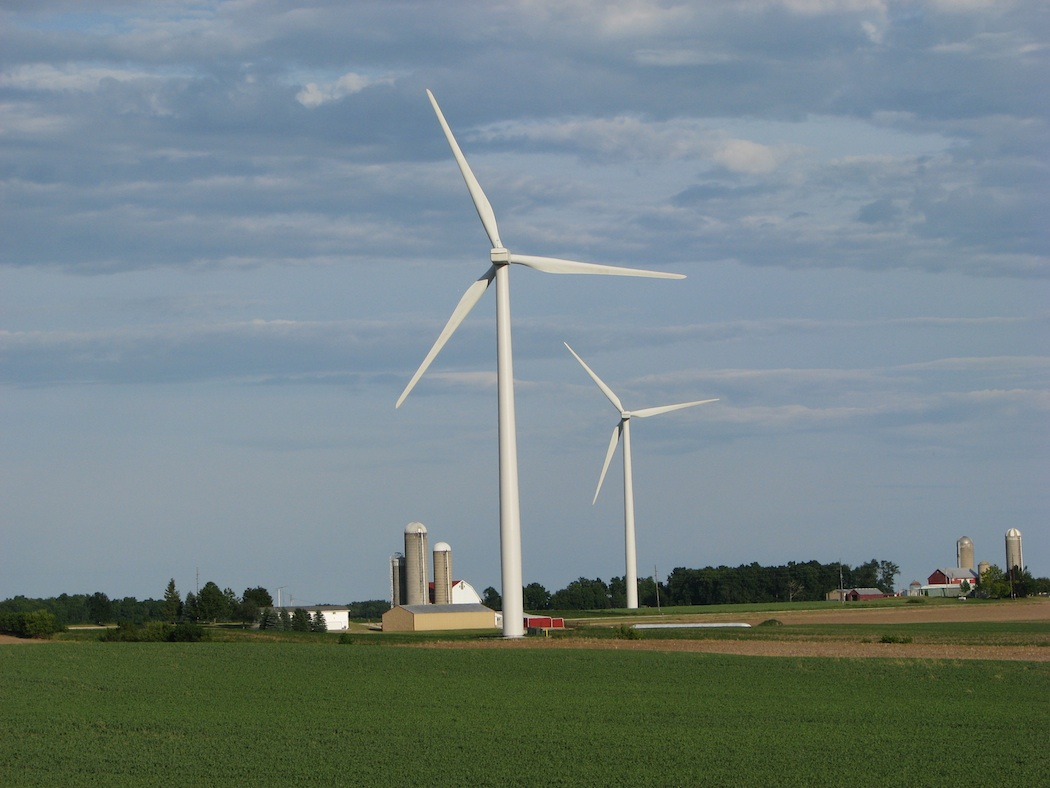
\includegraphics[height=2.5in]{files/21206}
            \caption{Wind turbines at the Forward Wind Energy Center in Fond du Lac and Dodge Counties, Wisconsin. (Photo by Ruth Baranowski / NREL)}\label{fig:21206}
          \end{subfigure}%
          \begin{subfigure}[b]{.5\linewidth}
            \centering
            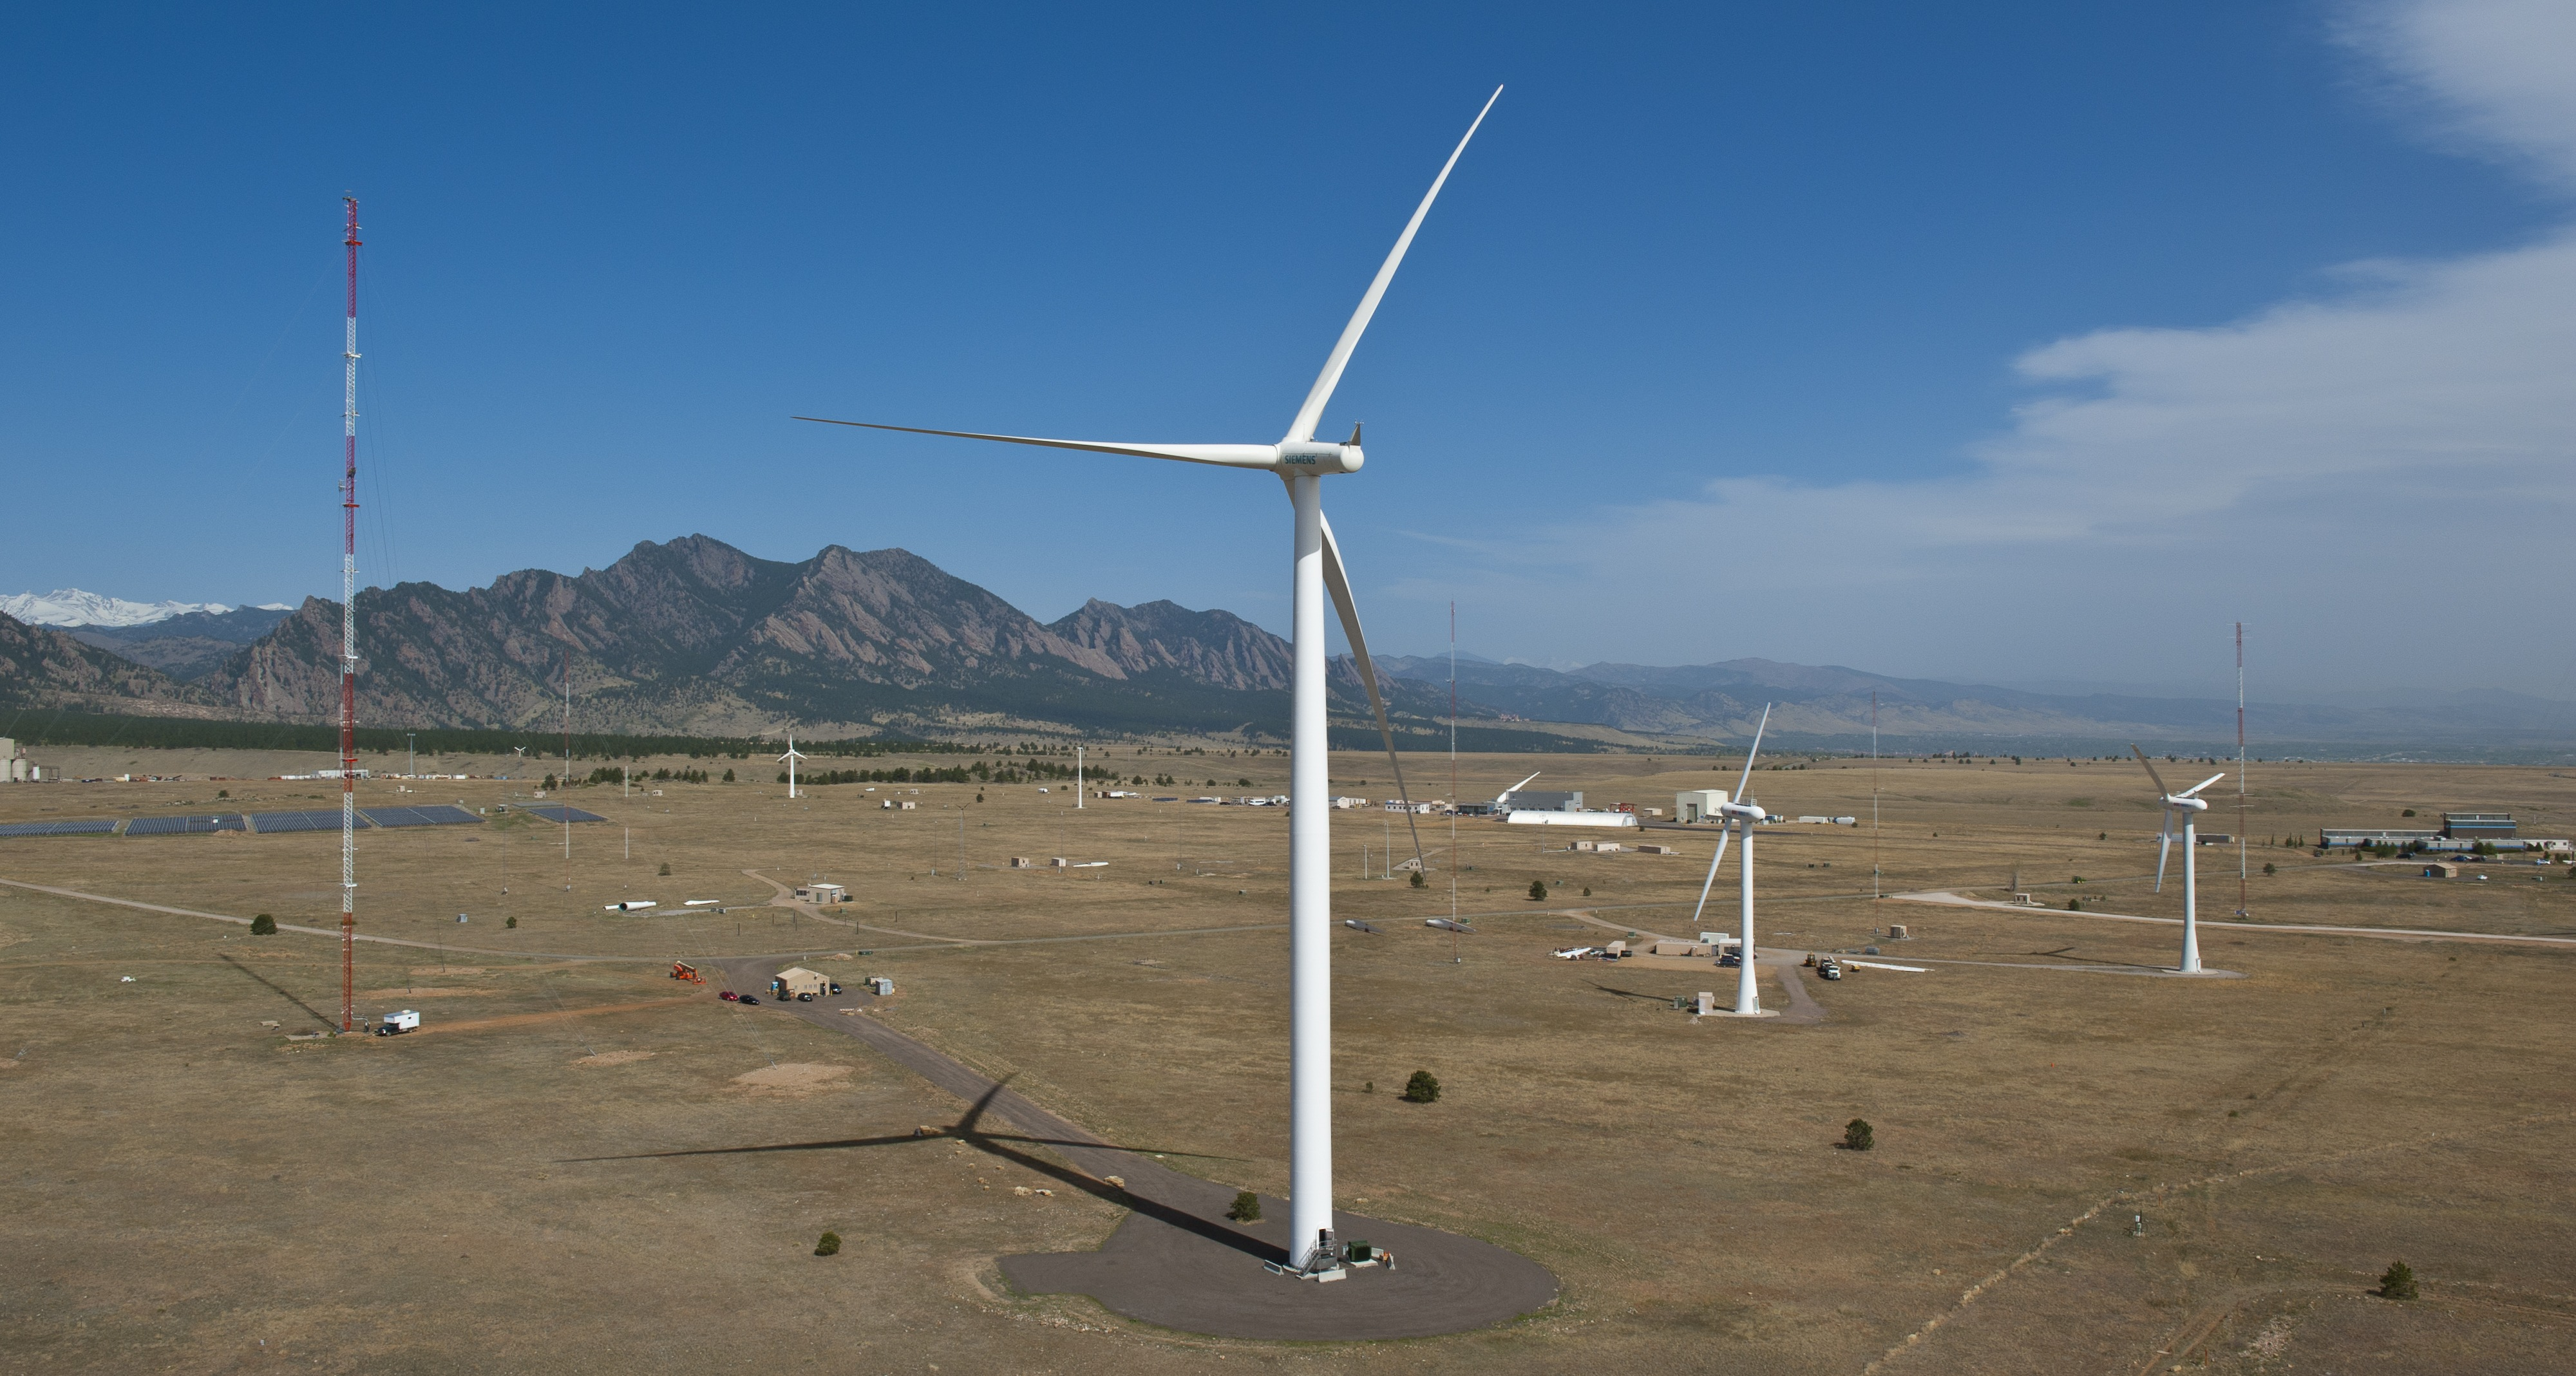
\includegraphics[height=2.5in]{files/20018}
            \caption{Aerial view of the National Wind Technology Center. (Photo by Dennis Schroeder / NREL)}\label{fig:20018}
          \end{subfigure}
          \caption{NREL images}\label{fig:NRELimages}
\end{figure}
\end{lstlisting}

Note that the \texttt{subfig} and \texttt{subfigure} packages are deprecated. The \texttt{subcaption} package appears to be the most frequently maintained package at this time, and contains the same functionality as the \texttt{subfig} and \texttt{subfigure} packages.

\begin{figure*}
          \begin{subfigure}[b]{.55\linewidth}
            \centering
            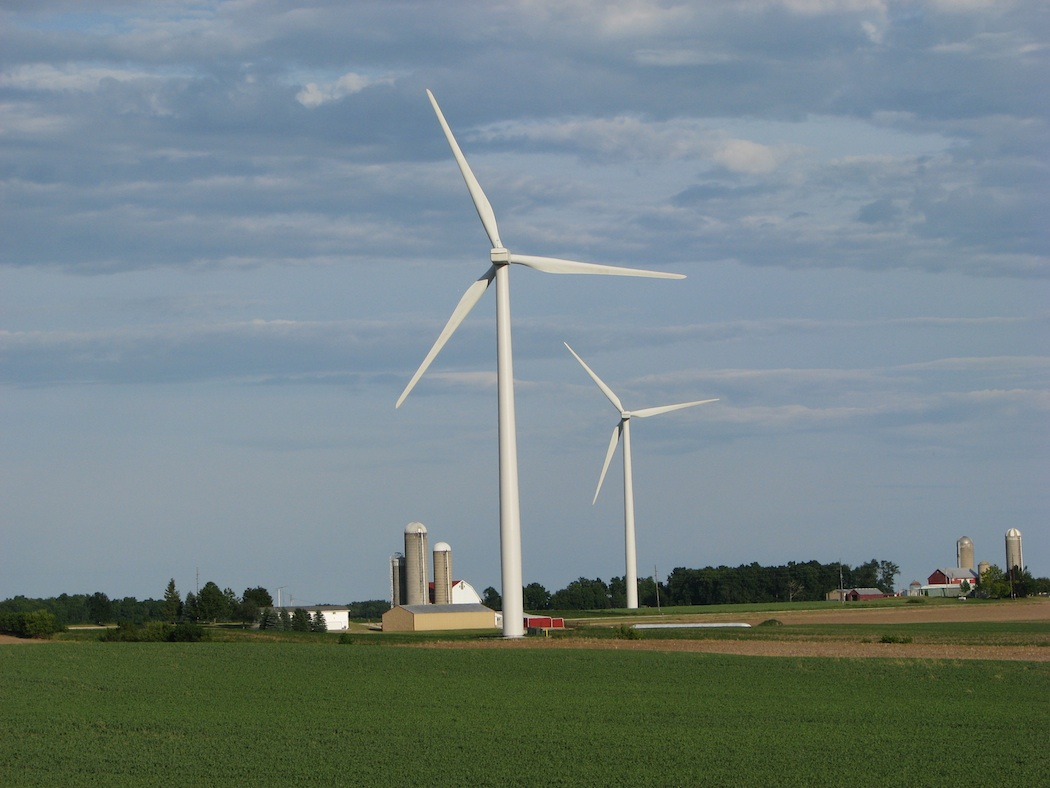
\includegraphics[height=2.5in]{files/21206}
            \caption{Wind turbines at the Forward Wind Energy Center in Fond du Lac and Dodge Counties, Wisconsin. (Photo by Ruth Baranowski / NREL)}\label{fig:21206}
          \end{subfigure}%
          \begin{subfigure}[b]{.55\linewidth}
            \centering
            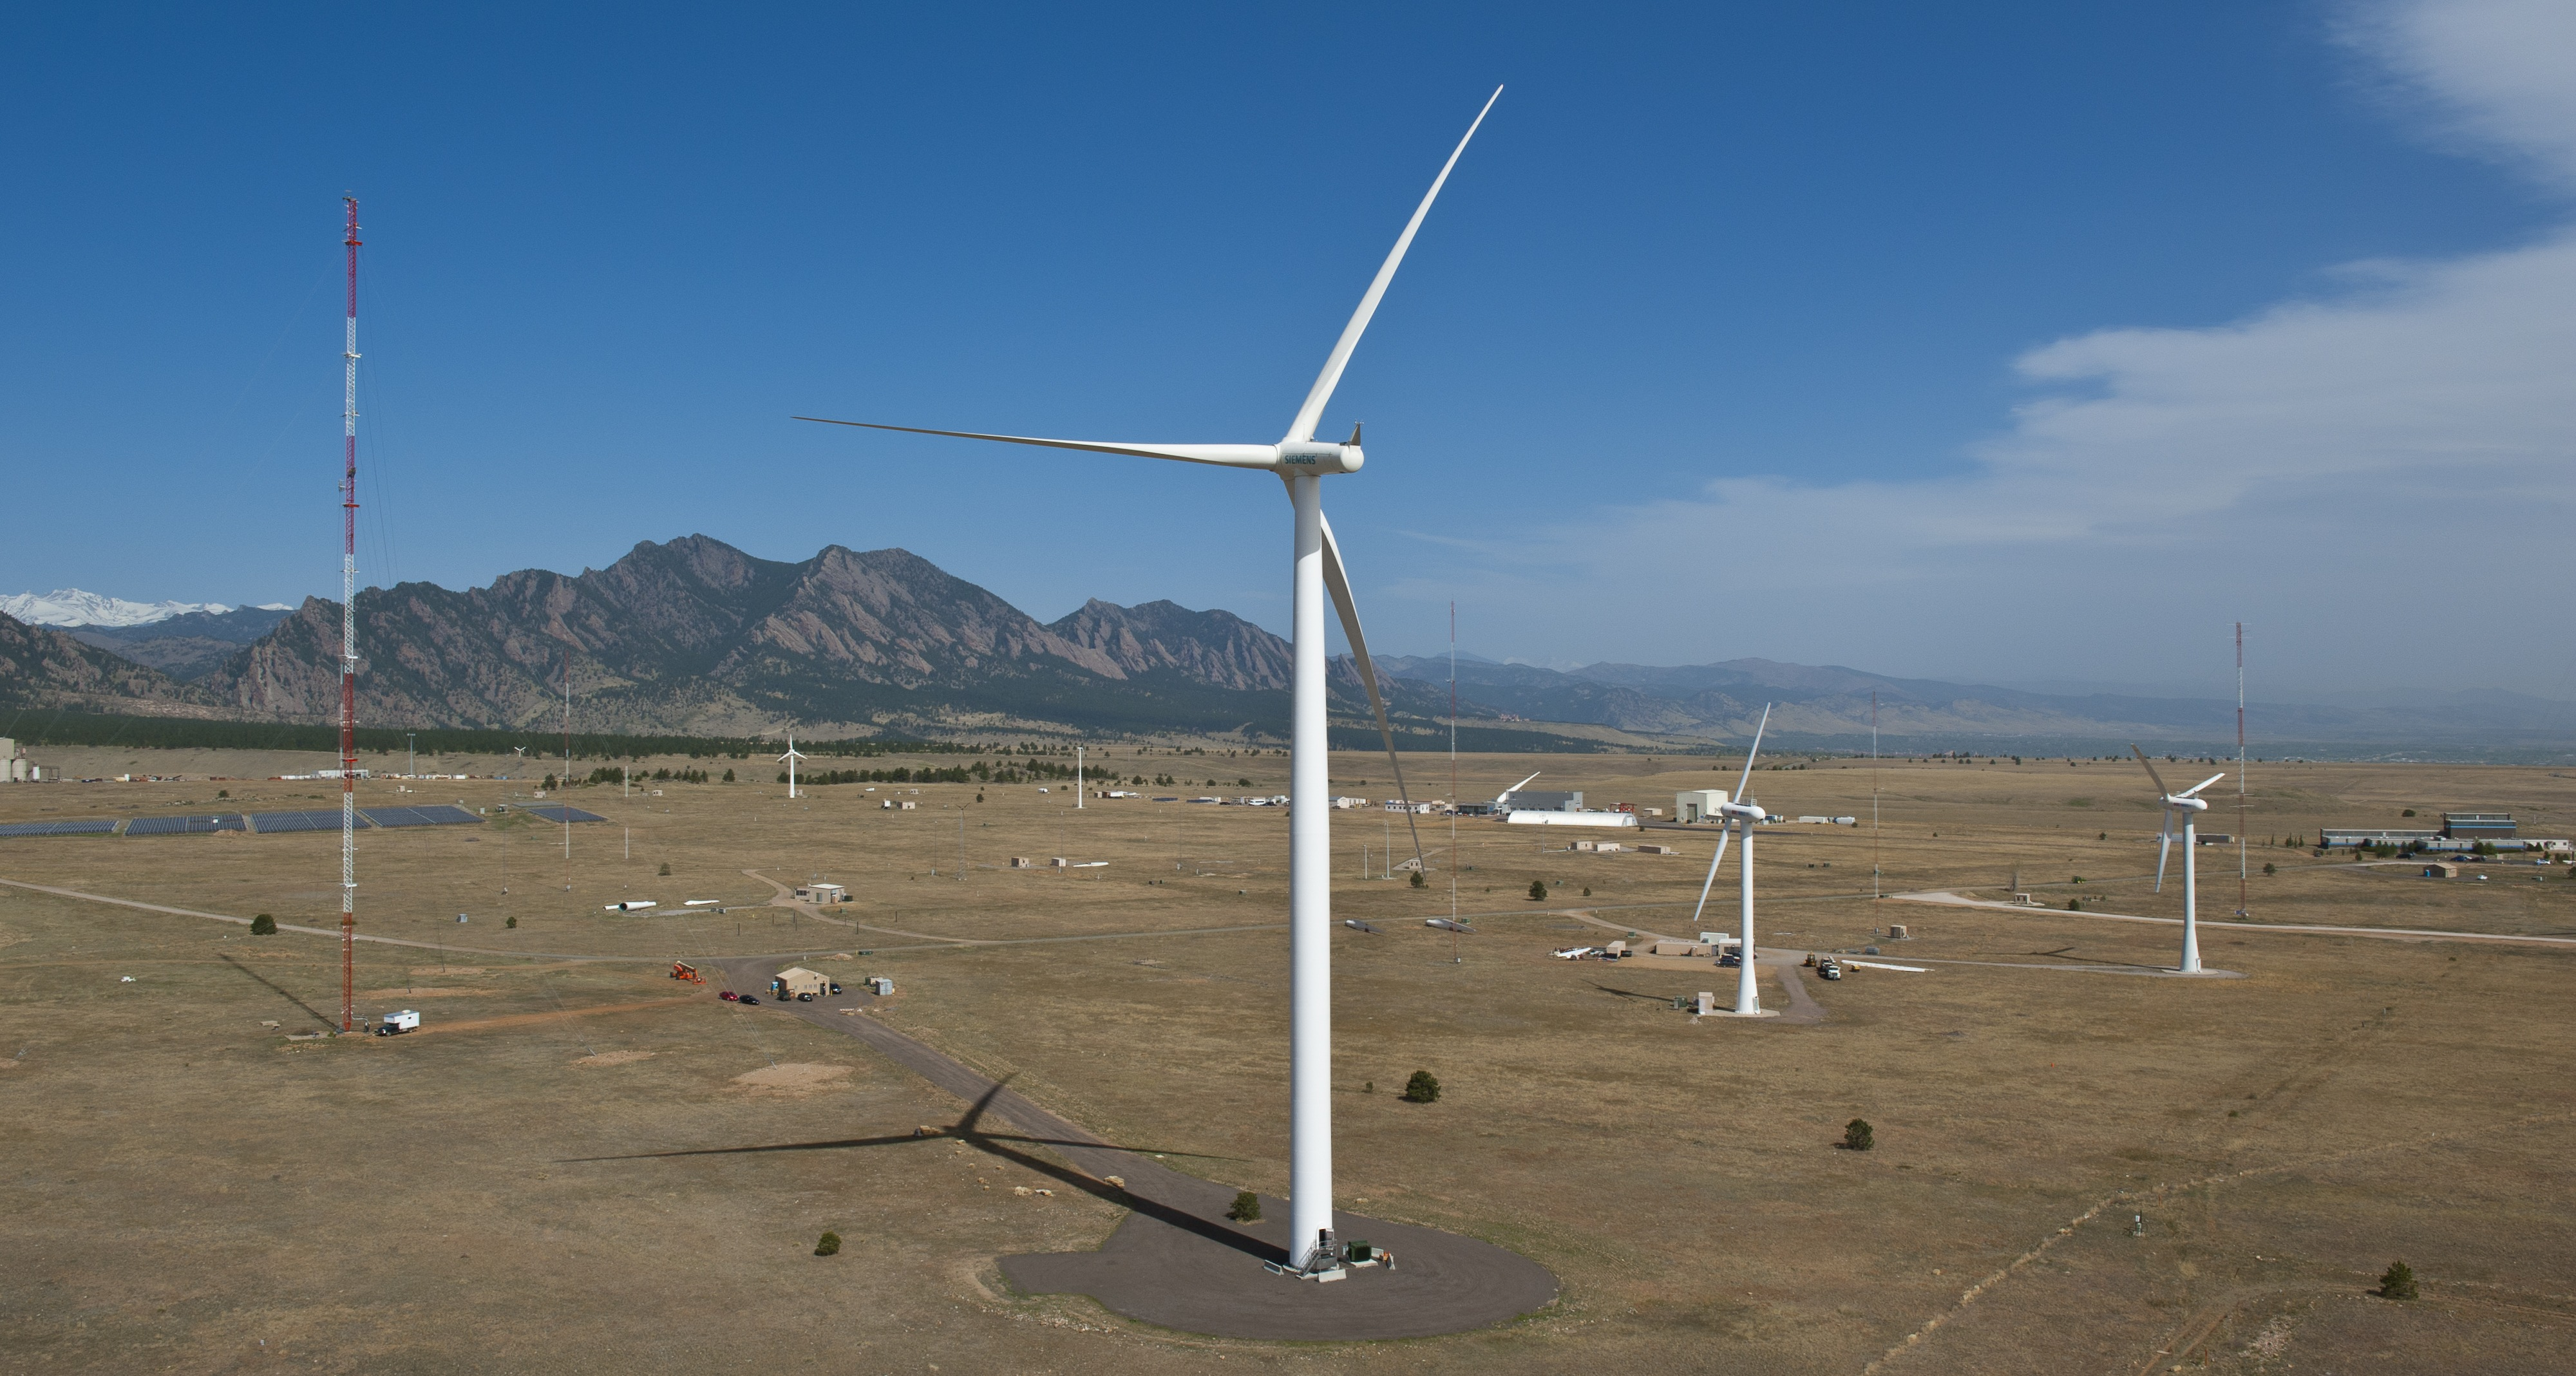
\includegraphics[height=2.5in]{files/20018}
            \caption{Aerial view of the National Wind Technology Center. (Photo by Dennis Schroeder / NREL)}\label{fig:20018}
          \end{subfigure}
          \caption{NREL images}\label{fig:NRELimages}
\end{figure*}

\subsection{Citations}
\label{Sec:Bib}
Use \texttt{bibtex} to organize references and store them in a single file (e.g. \verb+/Documents/bibliography/bibliography.bib+). The bibliography will then contain entries with `keys' for each source, like \texttt{Lamport\_1986\_a}. 

Authors can then insert citations to this key throughout their document, using different styles of citation. Citations are generated using the \texttt{biblatex} package, which also formats references in the correct style.  Ways to generate citations are described in the \texttt{biblatex} documentation, and include:
\begin{itemize}
\item \verb+\cite{Lamport_1986_a}+ prints \cite{Lamport_1986_a}.
\item \verb+\citep{Lamport_1986_a}+ prints \citep{Lamport_1986_a}.
\item \verb+\citet{Lamport_1986_a}+ prints \citet{Lamport_1986_a}.
\end{itemize}

To cite URLs, use the 'misc' style. For example, the bibtex entry for \href{http://tex.stackexchange.com}{http://tex.stackexchange.com}\ \cite{texstackexchange} looks like this:

\begin{lstlisting}
@misc{texstackexchange,
	Author = {Anon.},
	Howpublished = {Accessed July 21, 2014: \url{http://tex.stackexchange.com}},
	Title = {\TeX -- LaTeX Stack Exchange},
	Year = {2014}}
\end{lstlisting}

This format will allow you to include the date on which a URL was accessed.

The citations should work with journal articles \citep{Clifton_2013_a}, books \citep{Knuth_1984_a, Lamport_1986_a, chicago}, technical reports \citep{TechReportTest}, and URLs \citep{texstackexchange}. Any unknown publication types will be formatted using the `misc' type.

\subsection{Including computer code}
The \texttt{listings} package has been loaded. Note: this does not work if the `Draft' document option is used.

To change the syntax highlighting use \verb+\lstset{language=[dialect]language,columns=fullflexible,keepspaces=true}+ before each listing where the language changes. For more details see the \texttt{lstlisting} documentation.

\subsection{NREL-style bibliographies}
NREL uses "Chicago A" style-references. The \emph{nrel.cls} file uses Biblatex to produce these references automatically. 

To include a bibliography in the document give the bibliography file location in the preamble, and insert the bibliography at the appropriate location:

\begin{lstlisting}
% give the bibliography file location
\bibliography{files/bibliography.bib}
...
\begin{document}
...
% insert the bibliography into the document
\cleardoublepage
\label{sec:Bib}
\printbibliography
...
\end{document}
\end{lstlisting}

An example bibliography is included in this document on page \pageref{sec:Bib}.

\subsection{Footnotes}
Footnotes can be inserted using the \verb+\footnote{}+ command\footnote{like this}. Footnotes are numbered in the main matter\footnote{and like this as well}, and use daggers, etc instead of numers in the appendices.

\section{Creating a file structure}
\label{sec:FileStructure}
Your main file should be called \emph{main.tex}. This helps editors and coauthors identify where to start. Then, use \texttt{input} to import other files into your main file at compilation.

For example, each of the chapters in this report is in separate files, called \emph{WhatIsLatex} (Chapter 1), \emph{NRELRequirements.tex} (Chapter 2), \emph{LatexAtNREL.tex} (Chapter 3), and so-on. In the example available on Github, they are stored in the \emph{files} directory. \emph{main.tex} then looks like this:

\begin{lstlisting}
...
\begin{document}
% content
\chapter{What is LaTeX?}
LaTeX is a mark-up language that describes how a document should be prepared. Three things are needed to make a LaTeX document:
\begin{enumerate}
\item A source document, usually with extension \emph{.tex}
\item Some packages and classes that help turn what's in the source document into something helpful
\item A compiler, also referred to as a working LaTeX installation.
\end{enumerate}

At first glance the source document looks like a programming language, and that's because it is: LaTeX is not WYSIWYG, like many of the document preparation tools in common use today. A good analogy is html.

\section{Printed Resources}


\section{Online Resources}
The wikibook at \href{http://en.wikibooks.org/wiki/LaTeX}{http://en.wikibooks.org/wiki/LaTeX} is an excellent resource. There are also several internet forums such as \href{tex.stackexchange.com}{tex.stackexchange.com} that may be useful.

Documentation for the packages used in the nrel.cls file (Section \ref{sec:nrelcls}) can be found at \href{ctan.org}{ctan.org}.

\input{files/NRELRequirements}
\input{files/LatexAtNREL}
...
\end{lstlisting}

\section{Best practice in writing a document in LaTeX}
\begin{description}
\item[Create a structure before you get too far.] Authors will find it easier to write documents and make changes if they separate the content of the document from the structure.
\begin{enumerate}
\item Each new LaTeX document should be placed in it's own directory. 
\item Create a main LaTeX file that just contains the preamble, custom commands and uses \texttt{input} to call the content. See Section \ref{sec:FileStructure} for an example where each \texttt{chapter} is contained in its own file. In an article, each \texttt{section} could be contained in its own file.
\item Keep the number of packages used to a minimum. If authors feel that something is desperately missing, they can contact the maintainers of the \emph{nrel.cls} file. Not all packages can be used as they lack compatibility.
\end{enumerate}
\item[Focus on content, not appearance.] Don't spend hours trying to adjust fonts, headers or spacing between lines. 
\begin{enumerate}
\item The document produced should meet NREL's requirements if it is compiled using \emph{nrel.cls}. 
\item Don't throw in lots of \texttt{clearpage}s or other commands to push material around. LaTeX is designed to handle that. 
\item Resist the temptation to add or subtract space, change lengths or do other things to modify the layout. 
\item Write!
\end{enumerate}
\end{description}
